\section{Consensus in distributed \\ blockchains}

The idea behind Proof-of type systems is that whoever should be able to add the next block in the blockchain is chosen by proving the ownership of some kind of resource. This resource could be
something determined by computer hardware, like computing power in Proof-of-Work systems or hard drive capacity in Proof-of-Space systems, or it could be determined by some kind of stake ownership in
the system like in Proof-of-Stake systems. Below we will describe some of these systems and compare them to each other.

\subsection{Proof-of-Work}

The most commonly used consensus algorithm in blockchains is a so called Proof-of-Work (POW) algorithm. It was and is still being used as the consensus algorithm in the implementation of
Bitcoin,\cite{url:bitcoin} and other widely used cryptocurrencies like Litecoin and Dogecoin. The idea behind a POW algorithm is that the creator of the next block is chosen randomly among peers,
where the chance of creating a block is proportional to the amount of computing power invested by the peer. Usually this computing power is provided by solving some kind of mathematical puzzle.

\subsubsection{Requirements for POW systems}

The puzzle in this context is some kind of computationally expensive operation, which is usually based on some cryptographic operation. After finding a solution to the puzzle it is then added to the
newly created block by the peer which solved it, in order to proove to the other peers that the correct solution has been found. Therefore it should be computationally easy for the other peers to
check the correctness of the solution. The puzzle chosen for a POW system can and should have some properties. Firstly it should be computationally hard enough to ensure that a significant amount of
computational power should have to be expended to be able to solve it otherwise the purpose would be lost. On the other hand however it should also be computationally easy for others in the system to
check the correctness of a proposed solution. Additionally it should also be possible to adjust the difficulty of the puzzle. This is very important to make the system future proof and to account for
the predicted exponential increase in computing power over the years.\cite{url:moore_law} Additionally in the context of blockchains the difficulty of the puzzle should also account for a potential
increase in computing power within the network caused by the addition of more peers.\par Lastly there is also the consideration of the usefulness of the puzzle. In most existing implementations of POW
systems the puzzle which should be solved does not provide any purpose other than to prove the ownerhship of computational power. In other words the solution of the puzzle has no value other then
finding the creator of the next block and the expended computing power is could be considered to be wasted.\cite{url:pow_useless} There have been some propositions and implementations for "useful" POW
type systems. One example is the algorithm used in the cryptocurrency Primecoin. Primecoin uses a POW type system where a byproduct of the solution for the puzzle is the discovery of potentially new
prime numbers.\cite{url:primecoin} However this has some disadvantages, for example it is very hard to adjust the difficulty and therefore control the average time it takes to create a new block.

\subsubsection{Examples for existing POW systems}

The first kind of use for a POW type system was called Hashcash\cite{url:hashcash} and was created to combat spam emails and denial of service attacks. The idea of a system like Hashcash was firstly
proposed in 1992 by Cynthia Dwork and Noni Naor.\cite{url:pow_email} The concrete proposal for Hascash and its first implementation followed in 1997.\cite{url:hashcash} The basic idea behind Hashcash
is that the sender takes the header of the email he wants to send, appends a 20 bit long number at the end of it and computes the 160 bit long SHA-1 hash value of it. The goal is to find a hash in
which the first 20 bits are set to zero. If this is not the case the appended number is increased by one and the hash is computed again. This is done until a hash with the first 20 bits set to zero is
found. The email is then sent with the number which satisfies this condition appended to the header. The receiver of the email can then simply try to hash the header himself and he can immediately see
if the resulting hash satisfies the conditions. This system ensures that the sender has to expend some amount of computing power by hashing the header a significant amount of times until it fulfills
the condition. For the receiver however the check can be done immediately since he only has to compute the hash once. Ideally for the sender this means that he has to calculate for some amount of time
until he can send out the email which prevents the sending of a lot of potential spam emails at once. This system also accounts for the increase of computing power over the years since the difficulty
of the computation can be increased by increasing the required number of zero bits in the hash. However the only way to adjust the difficulty is by applying a software update, since the difficulty is
currently statically set to 20 bits.\par The first use of a POW system for the purpose of a consensus algorithms in a blockchain is however the one used for bitcoins. The idea is very similar to the
one used in Hashcash as both systems use a cryptographic hash function (SHA-256 in Bitcoin) with which they try to find a hash with a certain number of leading zeros, depending on the desired
difficulty. Instead of hashing the header of a email however, in Bitcoin the block which should be added to the chain is hashed. Similar to the Hascash system the block contains a number which is
increased until a valid hash is found. Among other things the new block also contains the hash of the previous block in the chain. This is necessary not only to ensure that the blocks are linked and
create a chain but also to make sure that someone can not try to find the hash for a future block in advance. 

\begin{figure}[ht]
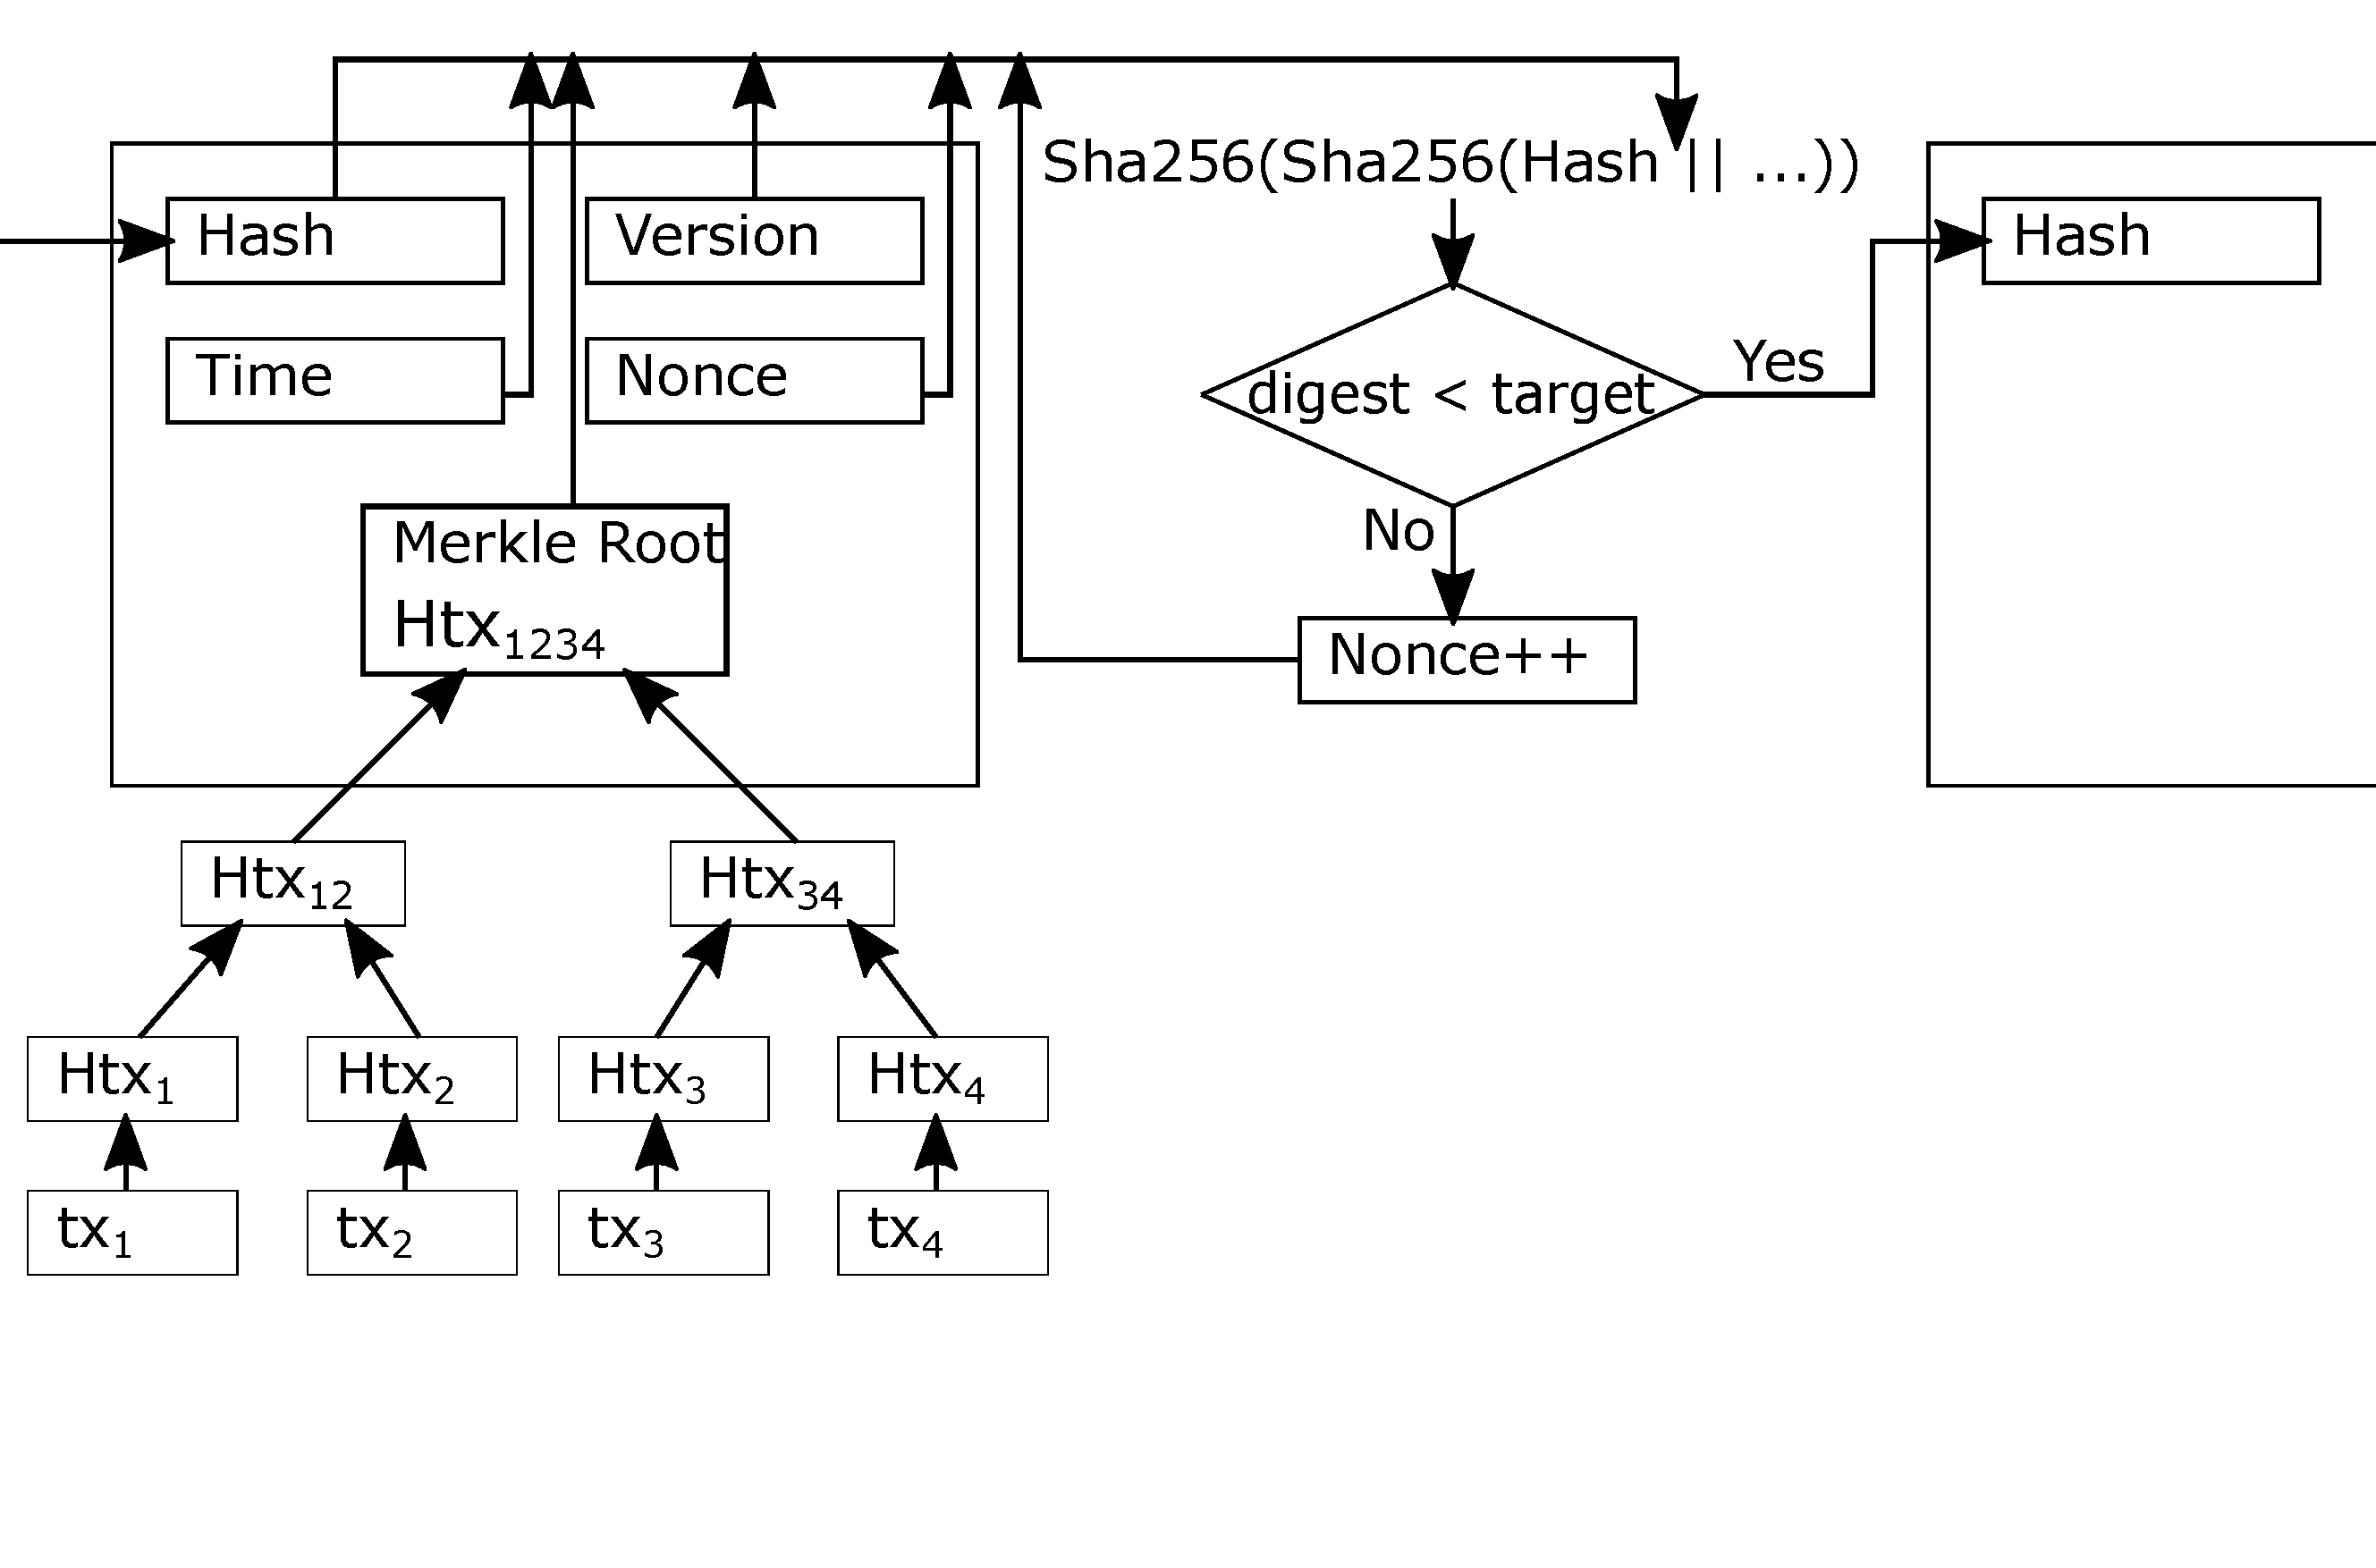
\includegraphics[width=1\columnwidth]{fig/btc.pdf}
\caption{Illustration of the Bitcoin mining algorithm}
\end{figure}

As with Hashcash the difficulty can be adjusted by adjusting the required number of
leading zeros in the hash. In the most cryptocurreny networks which use POW this difficulty adjusts itself such that the creation time of a new block is more or less constant. In the case of the
Bitcoin network the average creation time is 10 minutes. This whole system of trying to find a solution and then adding a block to the chain is called mining. To provide an incentive for people to
mine there is a reward of some amount of Bitcoins for whoever finds the next solution and adds the next block to the chain.\cite{url:bitcoin}\par Another type of POW algorithm used in cryptocurrencies
like Litecoin or Dogecoin is the so called scrypt algorithm.\cite{url:litecoin_dogecoin} The basic concept behind scrypt is that in the first step a large number of pseudorandom bit strings are
generated. The amount of these bit strings is such that it could very well be possible to run into memory limitations while trying to store all the strings. In a second step, these strings are then
accessed in pseudorandom order and used to generate a key. Since the execution of this algorithm is not only computationally hard but also has a significant memory requirement it could also be
categorised as a Proof-of-Space type algorithm\cite{url:scrypt} which is further explained in section \rec{proof-of-space}.

\subsubsection{Problems with POW systems}

One of the already mentioned problems with using POW as a consensus algorithm is the already mentioned fact that with most implementations the computing power expended could be considered to be wasted
especially considering the fact that there is a significant electrical power usage if the network reaches a certain size. In the example of the Bitcoin network this escalated to the point that the
power consumption of the entire bitcoin network is estimated to be at around 3 Gigawatts which is equivalent to the power consumption of the entire state of Morocco.\cite{url:btc_power}

Another problem which arouse after Bitcoin started to become popular, which is also a problem with other types of consensus algorithms is the fact that with a big enough investment it is possible to
overpower the rest of the network. Since the reward for mining is a significant amount of Bitcoins, a lot of people tried to earn money by using their PCs to mine. As more and more people joined the
mining network, the difficulty increased and more efficient ways of mining Bitcoins emerged. For this purpose Application Specific Integrated Circuits (ASICs) started to emerge. ASICs are basically
small circuits made for one special purpose. In the case of Bitcoins this purpose is to calculate SHA256 hashes as fast as possible.\cite{url:asic} These ASICs where a lot cheaper and more energy
efficient then PCs and started to make mining with them unprofitable. Soon even companies emerged which had bitcoin mining as their only business model. This happened especially in China, because both
the hardware and the electricity cost is comparably very low compared to other countries. This lead to the fact that today an estimated 71\% of the mining power comes from a few Chinese companies with
halls full of dedicated Bitcoin mining hardware. This lead to so called hash power centralization and therefore the loss of one of the core concepts of blockchains, namely the
decentralization.\cite{url:btc_china}

\subsection{Proof-of-Stake}

The idea behind a Proof-of-Stake (POS) type system is that instead of determining the peer which should be able to add the next block through computing power, as in POW systems, the peer is instead
selected by calculating some stake value first and then choosing a peer based on the highest stake in the network. There are various ways to calculate the required stake values, each with different
criteria. The trust from other peers in the network then comes from the fact that the peer with the highest stake has the highest incentive to add a block which is in agreement with the other peers.
Otherwise, if consensus is lost, then the trust in the network is lost as well and that peer loses the most since he has the highest stake. The idea was first proposed by the user QuantumMechanic in a
blog post.\cite{url:pos}

\subsubsection{Requirements for POS systems}

Some things have to be considered when trying to implement a POS type system. Firstly there should be a mechanism to ensure that a single peer is not able to create multiple blocks in a row, since
that would give it a control over the chain. Another problem which emerges when trying to implement a POS system is the resolution of so called forks in the blockchain. Forks happen quite frequently
in blockchains, when there is no clear consensus at one point in the network. There has to be a way to resolve such forks and to regain consensus in some way. In the case of POW systems this problem
is resolved by looking at the combined difficulty of the blocks in one of the forks. After some amount of time one of the forks will have a higher difficulty compared to the others and the peers will
then adopt the fork with the highest combined difficulty and drop all other forks.\cite{url:bitcoin} In the case of POS systems however if a fork happens and there is no single consensus, a peer has
nothing to loose by trying to follow both forks, which in turn means that regaining consensus is impossible. Different implementations have different ways of dealing with such a consensus
failure.\cite{url:pos_impossible}

\subsubsection{Examples of existing POS systems}

One example of a POS type systems can be found in the implementation of the cryptocurrency Nxt. In the Nxt network a peer is mining (often called forging in POS) by taking the generation signature
from the previous block in the chain and signing it with its own public key. The resulting 64-byte signature is then hashed using SHA256 and saved as an \textit{account hit}. This account hit is then
compared to the peers current target value and if the account hit is lower than the target value, the peer is validated to create the next block. The current target value is individual for each peer
and is calculated using the following formula: $$T=T_b*S*B_e$$ where $T$ is the new current target value of a peer, $T_b$ is a base target value which is constant for each block and calculated such
that the creation time of each block remains at a constant 60 seconds, $S$ is the time in seconds since the last block was created and $B_e$ is the account balance of the peer. As we can see the
target value increases every second, to ensure that the probability for a peer to get a account hit lower than the target value increases. The current target value is also higher for peers with a
higher account balance such that peers with a higher stake have a higher chance and we therefore get a POS system. The result of this algorithm is that a peer which owns 5\% of the coins in the
network should approximately be able to create 5\% of the blocks in the chain. To ensure that a single peer is unable to create multiple blocks in a row a peer is only allowed to mine if he did not
create one of the past 1440 blocks. Additionally a peer has to have owned its current coins for at least 1440 block before its stake is considered to ensure that a peer does not simply move his stake
between wallets and is therefore able to create multiple blocks in a row. The problem of consensus loss is solved similarly as with POW systems as each block has an assigned difficulty value based on
the target value of the creating peer.\cite{url:nxt}\par Another type of POS system was proposed during the creation of the cryptocurrency Ethereum. The so called Slasher algorithm, which was never
implemented in Ethereum, proposes an algorithm in which a peer that tries to follow two forks in the blockchain is being punished by the network. In short what happens is that if a peer tries to add a
block to both forks of the chain, then other peers which notice this behaviour can publish their finding to the network. The result is then that the \textit{cheating} peer loses its reward for adding
the block and the peer who found the "cheater" gets 33\% of the reward.\cite{url:eth_slash} This algorithm was however discarded by the Ethereum developers, since not all consensus problems could be
solved and the implementation of the punishing cheater algorithm by itself would be non-trivial.\cite{url:eth_no_slash} Ethereum instead now uses a POW type algorithm.\cite{url:eth_pow}\par Another
cryptocurrency which uses POS as a part of its consensus algorithm is Peercoin. Similarly to Nxt in Peercoin a stake is calculated for each peer. In comparison to Nxt however the age of a coin i.e.
the time a coin is in possession of a peer is also relevant for calculating a peers stake. The older a coin is, the higher its value. In the case of consensus failure consensus is then regained by
choosing the fork with the higher number of collective coin age.\cite{url:peercoin} One big criticism for Peercoin however is that it uses a periodical, centralized broadcast issued by the developers
of the cryptocurrency to checkpoint blocks in the chain. These checkpointed blocks and all blocks in the chain before it have to be considered valid by all peers. This however causes the whole
blockchain to be somewhat centralized. Most other implementation which use POS algorithms make use of a hybrid between POS and POW algorithms called Proof-of-Activity later described in section
\ref{poa}.

\begin{figure}[ht]
\center
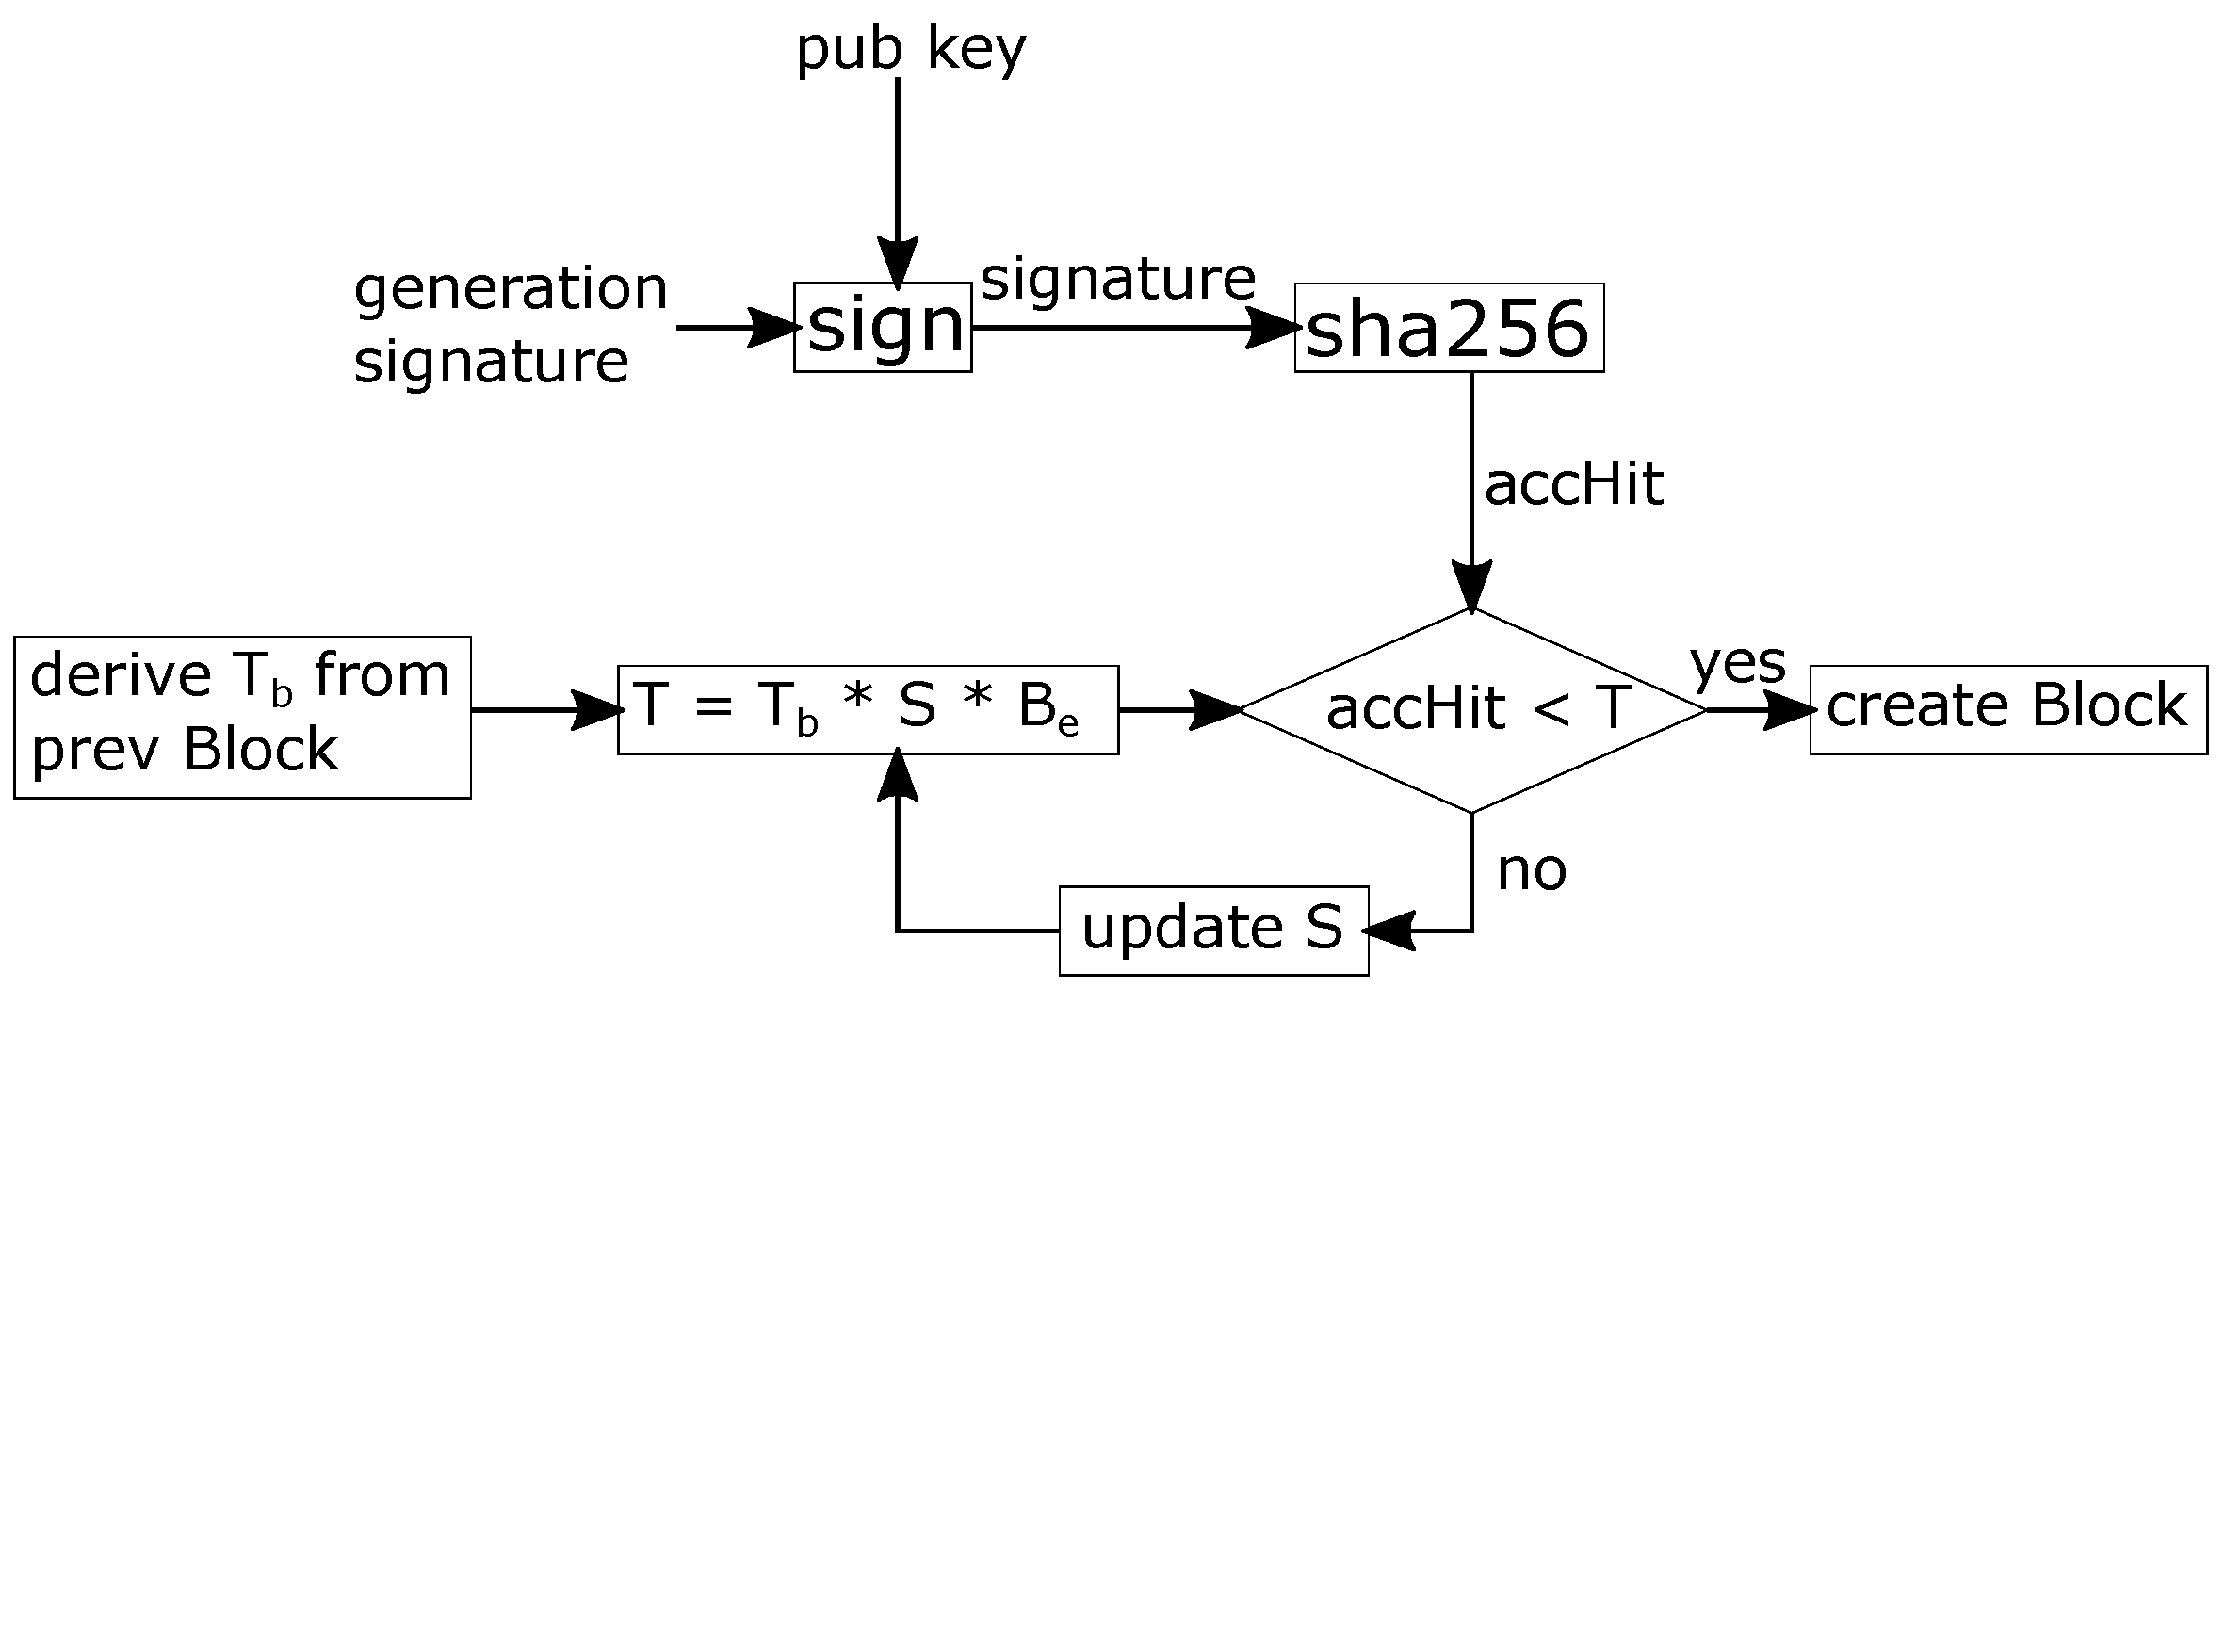
\includegraphics[width=1\columnwidth]{fig/PoS.pdf}
\caption{Nxts forging algorithm}
\end{figure}

\subsection{Proof-of-Activity} \label{poa}

Since both POW and POS type systems show some major disadvantages to each other, the idea of creating a hybrid between the two concepts emerged pretty soon. The idea is to use the properties of POW
systems to resolve consensus failures, while not having to solely rely on computational power to reach consensus.\par First we have to describe the so called \textit{follow-the-satoshi} subroutine
where a satoshi is the smallest possible unit of a cryptocurrency. Follow-the-satoshi selects a random peer in the network by taking a number between 1 and the total number of satoshis in the network
as input. This satoshi is then followed through the the blocks of the blockchain until it reaches the current owner which is then the selected owner for this satoshi. In this way the chance of beeing
the selected owner is higher if ones account balance is higher.\par The Proof-of-Activity (POA) mining protocol then works by walking through the following steps: 
\begin{itemize} 
\item A miner tries to find the valid hash value for the next block just like in POW systems and creates an empty block header if such a hash has been found. 
\item The header is then broadcast by the miner to the whole
network. 
\item Every peer then derives N stakeholders by concatenating the hash of the previous block with the hash in the new blocks header appending N fixed suffix values and hashing each
combination resulting in N different values which are then used to find N stakeholders by applying follow-the-satoshi. 
\item Every stakeholder who is online then checks if the new block header is
valid and whether he is one of the N derived stakeholders. If this is the case the peer signs the hash of the new block with its private key and broadcasts the signature. If the Nth stakeholder is
reached it includes some amount of transactions from the current transaction pool to the block as well as its own signature. 
\item The Nth stakeholder then broadcasts the block and all other peers can
check its validity by checking the validity of the hash in the header, derive all selected stakeholders and check their signatures. The reward for mining the block is then shared among the miner which
found the valid hash and all stakeholders which helped verifying the block. 
\end{itemize}

It is also important to add, that if some of the stakeholders are offline and therefore unable to sign the current block header, then after some time other miners will find different valid hashes
which will then derive different stakeholder until all selected stakeholders where able to add their signature.\cite{url:poa}

\subsection{Proof-of-Capacity or Proof-of-Space}

\label{proof-of-space}

A different kind of proposed consensus algorithm is the so called Proof-of-Capacity (POC), sometimes also referred to as Proof-of-Space, algorithm. The idea of POC is similar to the one used in POW,
but instead of using computational power as proof, disk space is used. This is done in order to reach consensus in a similar way to POW while being more ecologically friendly and fairer to smaller
peers, since disk space is less expensive compared to computational power and there is no danger for designated hardware to emerge for the sole purpose of mining.\par The basic concept of the POC
algorithm is that a peer generates some large data set in a predetermined way and stores it on his disk. If some other peer then wants to verify that the disk space is used he can ask for some
specific section of the generated data set, which the original peer can then provide. For this to work the generation of the data set has to be computationally expensive enough to ensure that the
proving peer cannot generate the data set on the fly and provide the requested subset, but has to actually keep it stored.\cite{url:poc}

\subsubsection{Existing POC systems}

For the most part the usage of POC has only been theorised. The only somewhat large scale implementation of a blockchain with POC as its consensus algorithm is with the cryptocurrency Burstcoin. In
its in 2014 released open implementation mining works in the following way: firstly every potential miner has to generate a large data set by taking his public address and a nonce and then applying a
hash function to it multiple times. The resulting data set is then called a plot. This plot is then divided into 4096 so called scoops and stored on the disk. This process of generating a plot and
storing it only has to be done once for every miner. After that mining works by firstly determining a scoop number which is derived from the previous block. The scoop with this scoop number is then
the only scoop relevant for the next block and is therefore the only scoop that has to be read from the whole dataset which is computationally very easy. The scoop is then hashed with the generation
signature of the next block. 8 bytes from the resulting hash are then taken and divided by a scaling factor, which can be adjusted and serves the same purpose as the difficulty in POW systems. The
result is then a number of seconds. If this number of seconds have passed since the generation of the last block then the user whose scoop was used to generate it is eligible to add the new block to
the chain. This way every user would be eligible if enough time passes.\cite{url:burstcoin}\par Other POC based cryptocurrencies like SpaceMint have also been proposed with similar algorithms but were
never fully implemented.\cite{url:spacemint}

\subsection{Proof-of-Burn}

Proof-of-Burn (POB) has been proposed as an alternative to POW systems. The way POB works is that to be able to start mining a peer has to "burn" some amount of coins first. Burning in this context
means that the coins are being sent to a address from which they are unretrievable and therefore lost forever. The more coins a miner sends to such an address the higher his chance becomes to be the
creator of the next block. The idea is that instead of spending money to buy mining hardware for POW systems, the money is instead directly burned skipping one step in between. For the purpose of
burning coins, coins from other cryptocurrencies can also be used. One major criticism for this concept is however that all current implementations only allow for the burning of currencies which use
the POW system. Which then nullifies the advantage POB would have over POW.\par The only at least somewhat active cryptocurrency currently using POB is Slimcoin\cite{url:pob}

\subsection{Proof-of-Elapsed-Time}

Proof-of-Elapsed-Time (POET) is another type of consensus algorithm proposed by Intel in 2015 as an alternative to POW. The idea is very similar to the one proposed by POW but instead of having to
expend computing power to solve a puzzle which takes approximately a predetermined amount of time, this time is just spend waiting instead of consuming computing power and therefore electrical power.
This provides some clear advantages. For once it is far more economical in comparison to POW. Secondly it provides a lot more fairness, since spending more money on hardware does not increase the
chance to be the one to validate a block. According to Intel it is also extremely efficient to implement such an algorithm using CPU level instructions already present on newer generations of Intel
CPUs. This however is also one of the major concerns of this proposed algorithm. By having to rely on Intel specific hardware, the whole system designed to be decentralized becomes very dependent on
Intel as a manufacturer, which is in contradiction to the idea of a blockchain in the first place.\cite{url:coinbase_consensus}\par The basic idea of the functionality of the algorithm is as follows:
the peers request a wait time from a so called enclave, which is just a function which is considered trustworthy by all peers which by Intels idea is present as a CPU instruction. The peer with the
lowest wait time is then the one who is validated by the other peers in the network for whatever operation he wants to do, in the case of a blockchain this would be to create a new block. The other
peers have to then be able to check, that the timer the validated peer used as a wait time is a valid timer he got from the trusted enclave. This can again be done by all peers through the
enclave.\par There is currently no real application using this algorithm, but Intel released an open-source implementation of such an algorithm which can be used for testing.\cite{url:poet}
